\documentclass[10pt,landscape]{article}
\usepackage{multicol}
\usepackage{calc}
\usepackage{ifthen}
\usepackage[landscape]{geometry}
\usepackage{listings}
\usepackage{amsmath,amsthm,amsfonts,amssymb}
\usepackage{mathtools}
\usepackage{color,graphicx,overpic}
\usepackage{hyperref}
\usepackage[dvipsnames]{xcolor}

\usepackage{MnSymbol}
\usepackage{graphicx}
\usepackage{wrapfig}

% This sets page margins to .1 inch if using letter paper, and to 1cm
% if using A4 paper. (This probably isn't strictly necessary.)
% If using another size paper, use default 1cm margins.
\ifthenelse{\lengthtest { \paperwidth = 11in}}
    { \geometry{top=0.2in,left=0.2in,right=0.2in,bottom=0.2in} }
    {\ifthenelse{ \lengthtest{ \paperwidth = 297mm}}
        {\geometry{top=1cm,left=1cm,right=1cm,bottom=1cm} }
        {\geometry{top=1cm,left=1cm,right=1cm,bottom=1cm} }
    }

% Turn off header and footer
\pagestyle{empty}

% Redefine section commands to use less space
\makeatletter
\renewcommand{\section}{\@startsection{section}{1}{0mm}%
                                {-1ex plus -.5ex minus -.2ex}%
                                {0.5ex plus .2ex}%x
                                {\normalfont\large\bfseries}}
\renewcommand{\subsection}{\@startsection{subsection}{2}{0mm}%
                                {-1ex plus -.5ex minus -.2ex}%
                                {0.5ex plus .2ex}%
                                {\normalfont\normalsize\bfseries}}
\renewcommand{\subsubsection}{\@startsection{subsubsection}{3}{0mm}%
                                {-1ex plus -.5ex minus -.2ex}%
                                {0.5ex plus .2ex}%
                                {\normalfont\small\bfseries}}
\makeatother

% Itemize to use less space
\usepackage{enumitem}
\setlist{leftmargin=*, nosep}
\setenumerate{nosep}

% Define BibTeX command
\def\BibTeX{{\rm B\kern-.05em{\sc i\kern-.025em b}\kern-.08em
    T\kern-.1667em\lower.7ex\hbox{E}\kern-.125emX}}

% Don't print section numbers
\setcounter{secnumdepth}{0}


\setlength{\parindent}{0pt}
\setlength{\parskip}{0pt plus 0.5ex}

%My Environments
\newtheorem{example}[section]{Example}

\newcommand{\Blue}[1]{\noindent{\textbf{\textcolor{Blue}{#1 -}}}}
\newcommand{\Red}[1]{\noindent{\textbf{\textcolor{BrickRed}{#1 -}}}}
\newcommand{\Green}[1]{\noindent{\textbf{\textcolor{PineGreen}{#1 -}}}}
\newcommand{\Hint}[1]{\noindent{\textcolor{Orange}{#1}}}
% -----------------------------------------------------------------------

\begin{document}
\raggedright
\footnotesize
\begin{multicols}{4}


% multicol parameters
% These lengths are set only within the two main columns
%\setlength{\columnseprule}{0.25pt}
\setlength{\premulticols}{1pt}
\setlength{\postmulticols}{1pt}
\setlength{\multicolsep}{1pt}
\setlength{\columnsep}{2pt}

\section{Linear Regression}

Linear regression means the dependent variable is \Hint{linear in the model coefficients}.

\begin{itemize}
    \item Linear: $y = b_0 + b_1 x_1 + b_2 x_2$
    \item Not linear: $y = b_0 x_1^{b_1} + b_3 x_2^{b_2}$
\end{itemize}

\subsection{\texttt{lm} in R}

\lstset{breaklines=true}

Rentals as a function of temperature and humidity:

\begin{lstlisting}[language=R]
mod <- lm(data = df, rentals ~ temp + rel_humidity)
summary(mod)
\end{lstlisting}

\subsection{Consider a ``Best Fitting'' Line}
\begin{displaymath}
    \boxed{
        \hat{y} = b_0 + b_1 x
    }
\end{displaymath}

\Blue{Slope $b_1$} sign is same as the sign of $\text{CORR}(X,Y)$. $\text{CORR}(X,Y)$ is between $[-1,1]$ and unit-less.
But $b_1$ has units.

\begin{displaymath}
    b_1 = \frac{\sum_{i=1}^{n} (x_i - \bar{x})(y_i - \bar{y})}{\sum_{i=1}^{n} (x_i - \bar{x})^2} = \text{CORR}(X,Y) \cdot \frac{\text{SD}(Y)}{\text{SD}(X)}
\end{displaymath}

\Blue{Intercept} $b_0 = \bar{y} - b_1 \bar{x}$

\Red{Mean-center data} if both $y$ and $x$ variables are mean-centered, rerun linear regression to get:

\begin{displaymath}
    \hat{y}_i - \bar{y} = b_1 (x_i - \bar{x})
\end{displaymath}

\begin{itemize}
    \item new intercept will be $0$
    \item new slope remains $b_1$
\end{itemize}

\Green{Regression to the mean} If $x = \bar{x}$ (the average of all $x$ values), the predicted $\hat{y} = \bar{y}$
(average of all $y$ values), \Hint{independent from $x$}.

\subsection{Independent Variables}

\Red{Categorical variables (``factor variable'' in R)} if encoded with one-hot, one category should be dropped to avoid perfect multicollinearity
(a situation where one predictor variable can be perfectly predicted from the others). This omitted category serves as a
reference category against which the other categories are compared. This approach is known as creating "dummy
variables."

\subsection{Evaluation}

\Blue{Residuals (error)} $e_i = y_i - \hat{y}_i$

\Blue{Sum of Squared Residuals}
\begin{displaymath}
SSR = \sum_{i=1}^{n} e_i^2 = \sum_{i=1}^{n} (y_i - \hat{y}_i)^2
\end{displaymath}

\Blue{Total Sum of Squares} a measure of the total variability in the observed data.
\begin{displaymath}
SST = \sum_{i=1}^{n} (y_i - \bar{y}_i)^2
\end{displaymath}

\Red{$R^2$} the \underline{proportion reduction} in sum of squared residuals by the regression model compared to the
baseline model (which always predicts the average value of all $y$s in the data: $\hat{y} = \bar{y}$).

\begin{displaymath}
    \boxed{
        R^2 = 1 - \frac{SSR}{SST} = \frac{SST - SSR}{SST}
    }
\end{displaymath}

\begin{itemize}
    \item $R^2$ of a regression model lies \Hint{between 0 and 1}.
    \item Adding a new independent variable to a regression model \Hint{can only increase $R^2$}.
    \item $R^2$ on its own cannot judge how good a model is.
\end{itemize}

\Green{$R^2$ in multiple linear regression} equals the
\Hint{square of the correlation between the \underline{actual values $y$} and the \underline{predicted values $\hat{y}$}}.
\begin{displaymath}
    R^2 = \left(\text{CORR}(y, \hat{y})\right)^2
\end{displaymath}
In the case of a perfect fit where every prediction of $y_i$ is going to be correct, then $R^2 = 1$

\Green{$R^2$ in simple linear regression} equals the
\Hint{square of correlation between dependent variable $y$ and independent variable $x$}.
\begin{displaymath}
    R^2 = \left(\text{CORR}(y, x)\right)^2
\end{displaymath}

\Blue{Degrees of Freedom} the number of observations minus the number of parameters estimated (including the intercept): $df = n - p - 1$

\Blue{Residual Variance} $\frac{SSR}{df}$

\Blue{Residual Standard Error} provides a measure of the average distance that the observed values fall from the
regression line.
\begin{displaymath}
RSE = \sqrt{\frac{SSR}{df}}
\end{displaymath}
\begin{itemize}
    \item Smaller RSE: the model's predictions are closer to the actual data points, suggesting a good fit.
    \item Larger RSE: the model's predictions are further from the actual data points, suggesting a poor fit.
\end{itemize}

\subsection{Troubleshooting}

The model's ability to predict the future and its interpretability can be impaired by

\begin{itemize}
    \item The presence of \underline{irrelevant} independent variables
    \item The presence of \underline{highly correlated} independent variables
    \item The presence of \underline{``too many''} variables relative to the size of the dataset
\end{itemize}

\Blue{\underline{Irrelevant} variables} have large p-values. Smaller p-value (R: \texttt{Pr(>|t|)}), the better. If
\Hint{lower than 0.05}, consider it \Hint{significant} at the 5\% significance level; otherwise, consider it
non-significant at the 5\% significance level. In R, a variable with \Hint{one or more \texttt{*} is considered
significant at 5\% level. A variable not significant at the 5\% level but at the 10\% level can be stated as ``less
clear''.}

\Green{p-value of a variable $x_i$} the probability of observing a coefficient estimate as extreme, or more extreme,
than the one actually obtained by the regression run in a similar sample \underline{assuming} $\beta_i = 0$.

\Blue{\underline{Highly correlated} variables} Detected by inspecting the correlation matrix. (R: \texttt{cor(df)}).

\Green{Multicollinearity} When two variables are highly correlated (typically correlations \Hint{higher than 0.75} in
magnitude), resolve this by removing either of the independent
variables and \underline{running the linear regression \textbf{again}}.

\Blue{Overfitting (\underline{``too many''} variables)} leads to poorly predicting future data. Remedy by (1) avoiding
``non-significant'' variables uising the starts \texttt{*} as a guide and (2) out-of-sample testing.

\Green{Out-of-Sample Testing}
\begin{enumerate}
    \item Partition data set into 70\% trainning set and 30\% test set before creating the regression model.
    \item Generate a set of models (e.g. with different sets of variables) using \underline{only} the training data.
    \item Evaluate models on the \underline{test set} using \Hint{out-of-sample $R^2$}.
\end{enumerate}

\Green{Out-of-Sample $R^2$}
\begin{displaymath}
\boxed{
\begin{split}
        &\text{OSR}^2 = \\
        &1 - \frac{\text{SSR of regression model applied to the test set}}{\text{SSR of baseline model applied to the test set}}
\end{split}
}
\end{displaymath}

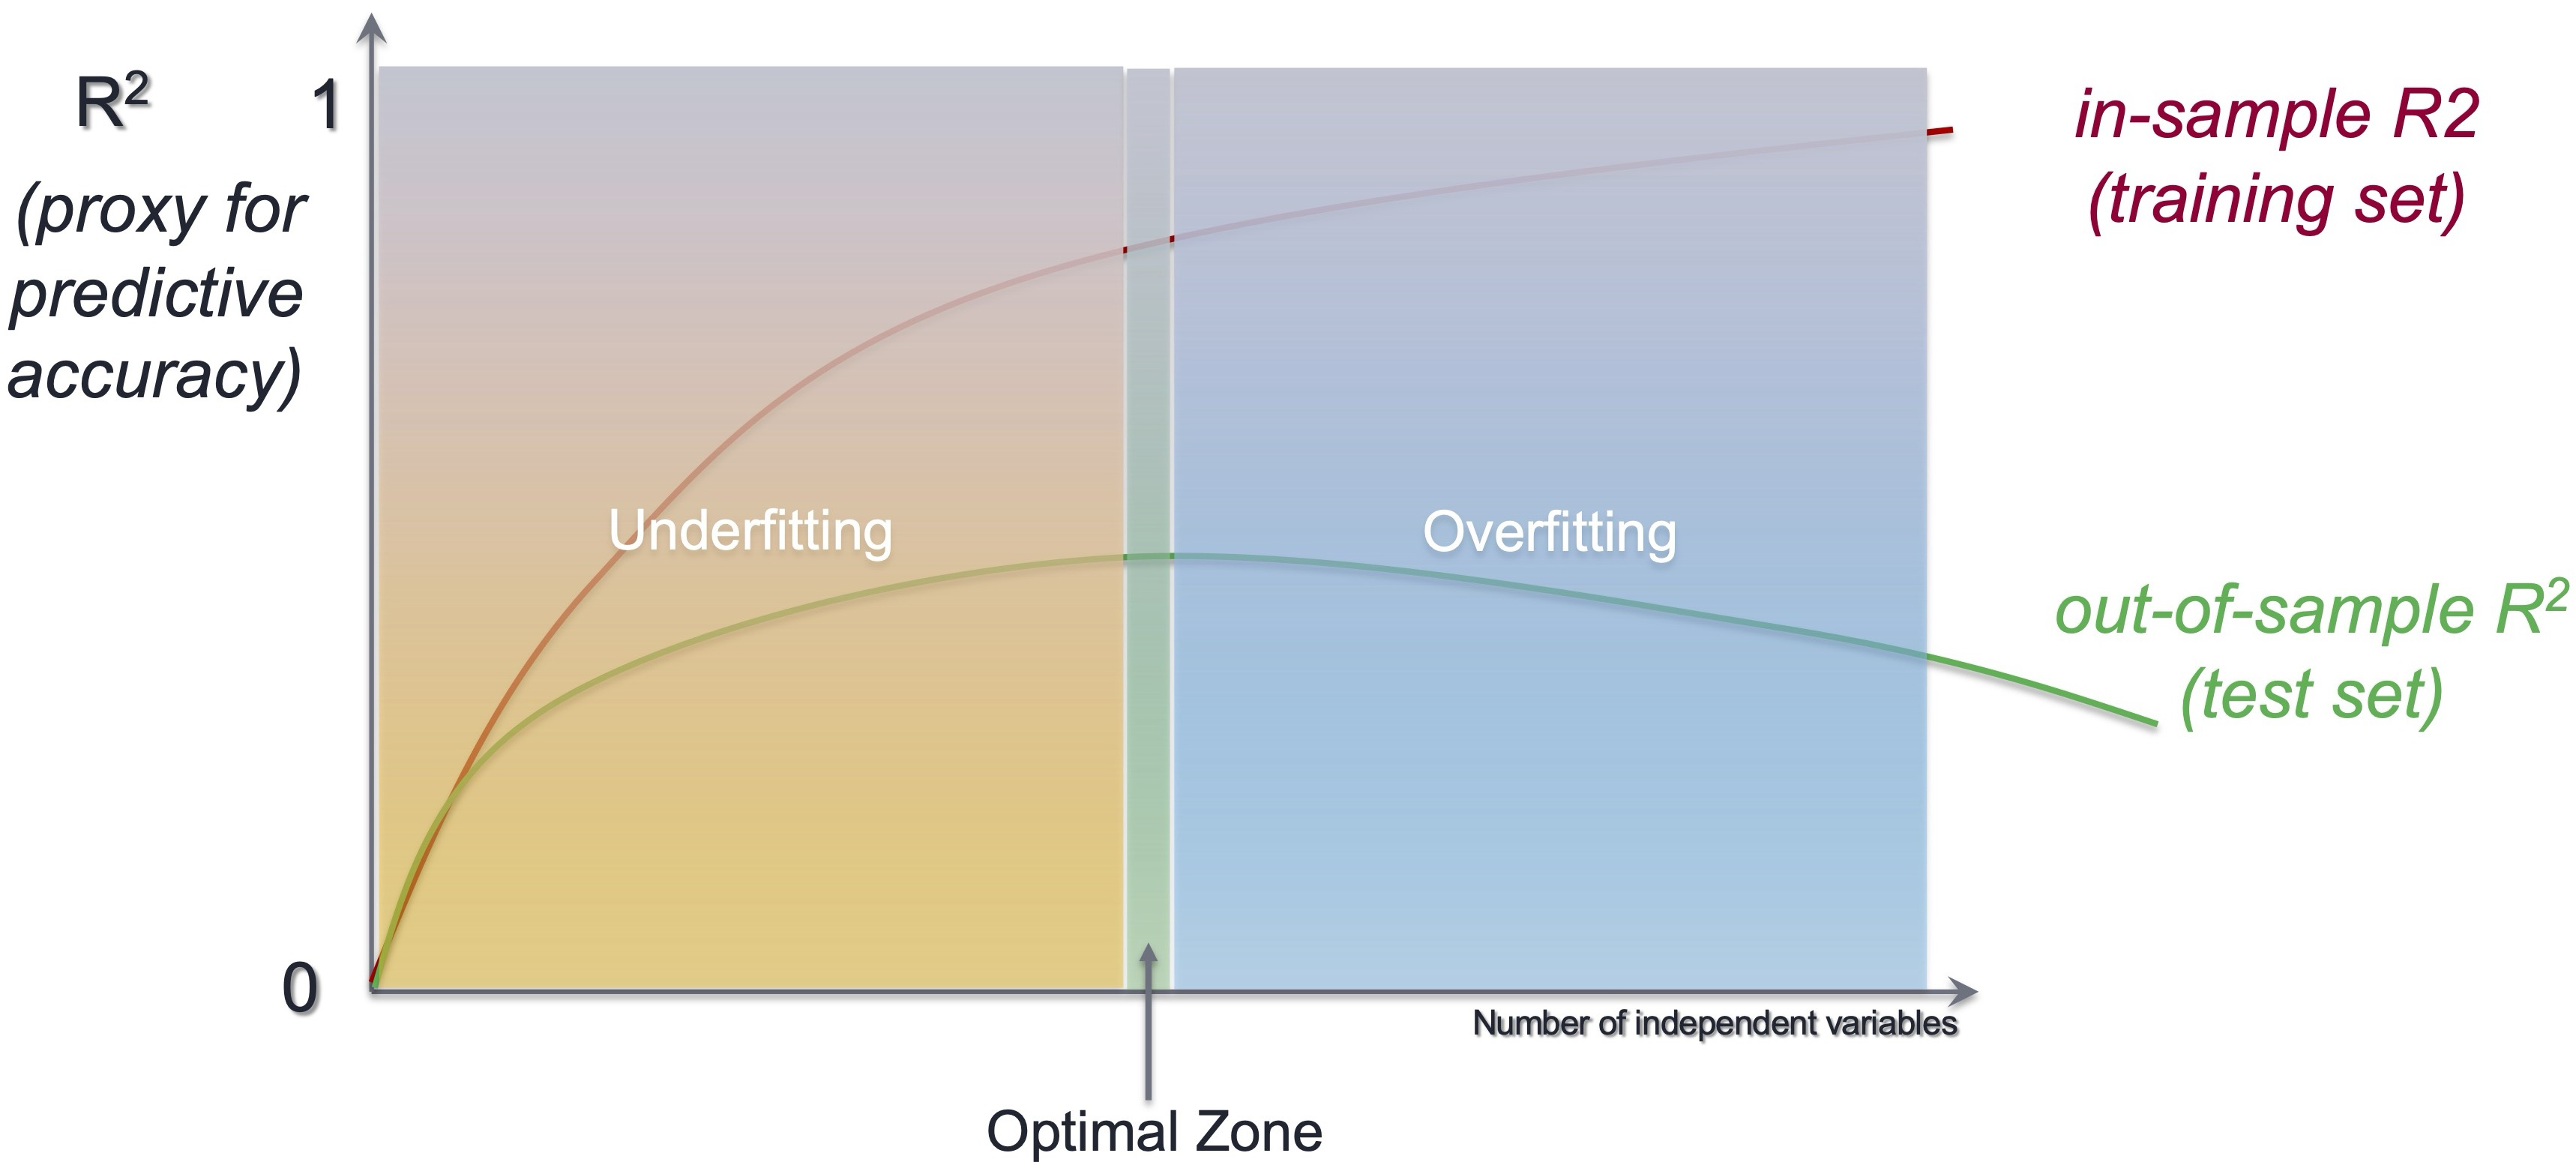
\includegraphics[width=0.25\textwidth]{overfitting.jpg}

\Red{Key takeaways}

\begin{itemize}
    \item Choose final model based on \underline{out-of-sample} predictive quality metrics.
    \item Use metrics like $R^2$ and the standard error of regression \underline{in combination} because they have different strength and weaknesses.
    \item Only include significant variables that are not highly correlated.
    \item Coefficients should ``make sense''.
    \item Use for interpolation rather than extrapolation.
\end{itemize}

\Blue{Inferring model's coefficient} from the practice: ``Correlation is not the same as causation. It could be that
individuals with other contributing factors happen to sleep longer. It could be that these other factors, not sleep per
se, are causally linked to the condition under study.''

\Red{Technical caution} for the p-value to be correct, the ``unaccounted for'' differences in the regression model
$\epsilon$ (think of the residuals) needs to have zero mean, constant standard deviation, be independent and follow a normal distribution.

\Green{Linearity} there is no curvature
\Green{Homoskedasticity} the dispersion of $e_i = y_i - \hat{y}_i$ is not systematically smaller or larger for large
$x_i$ values compared to small $x_i$ values.
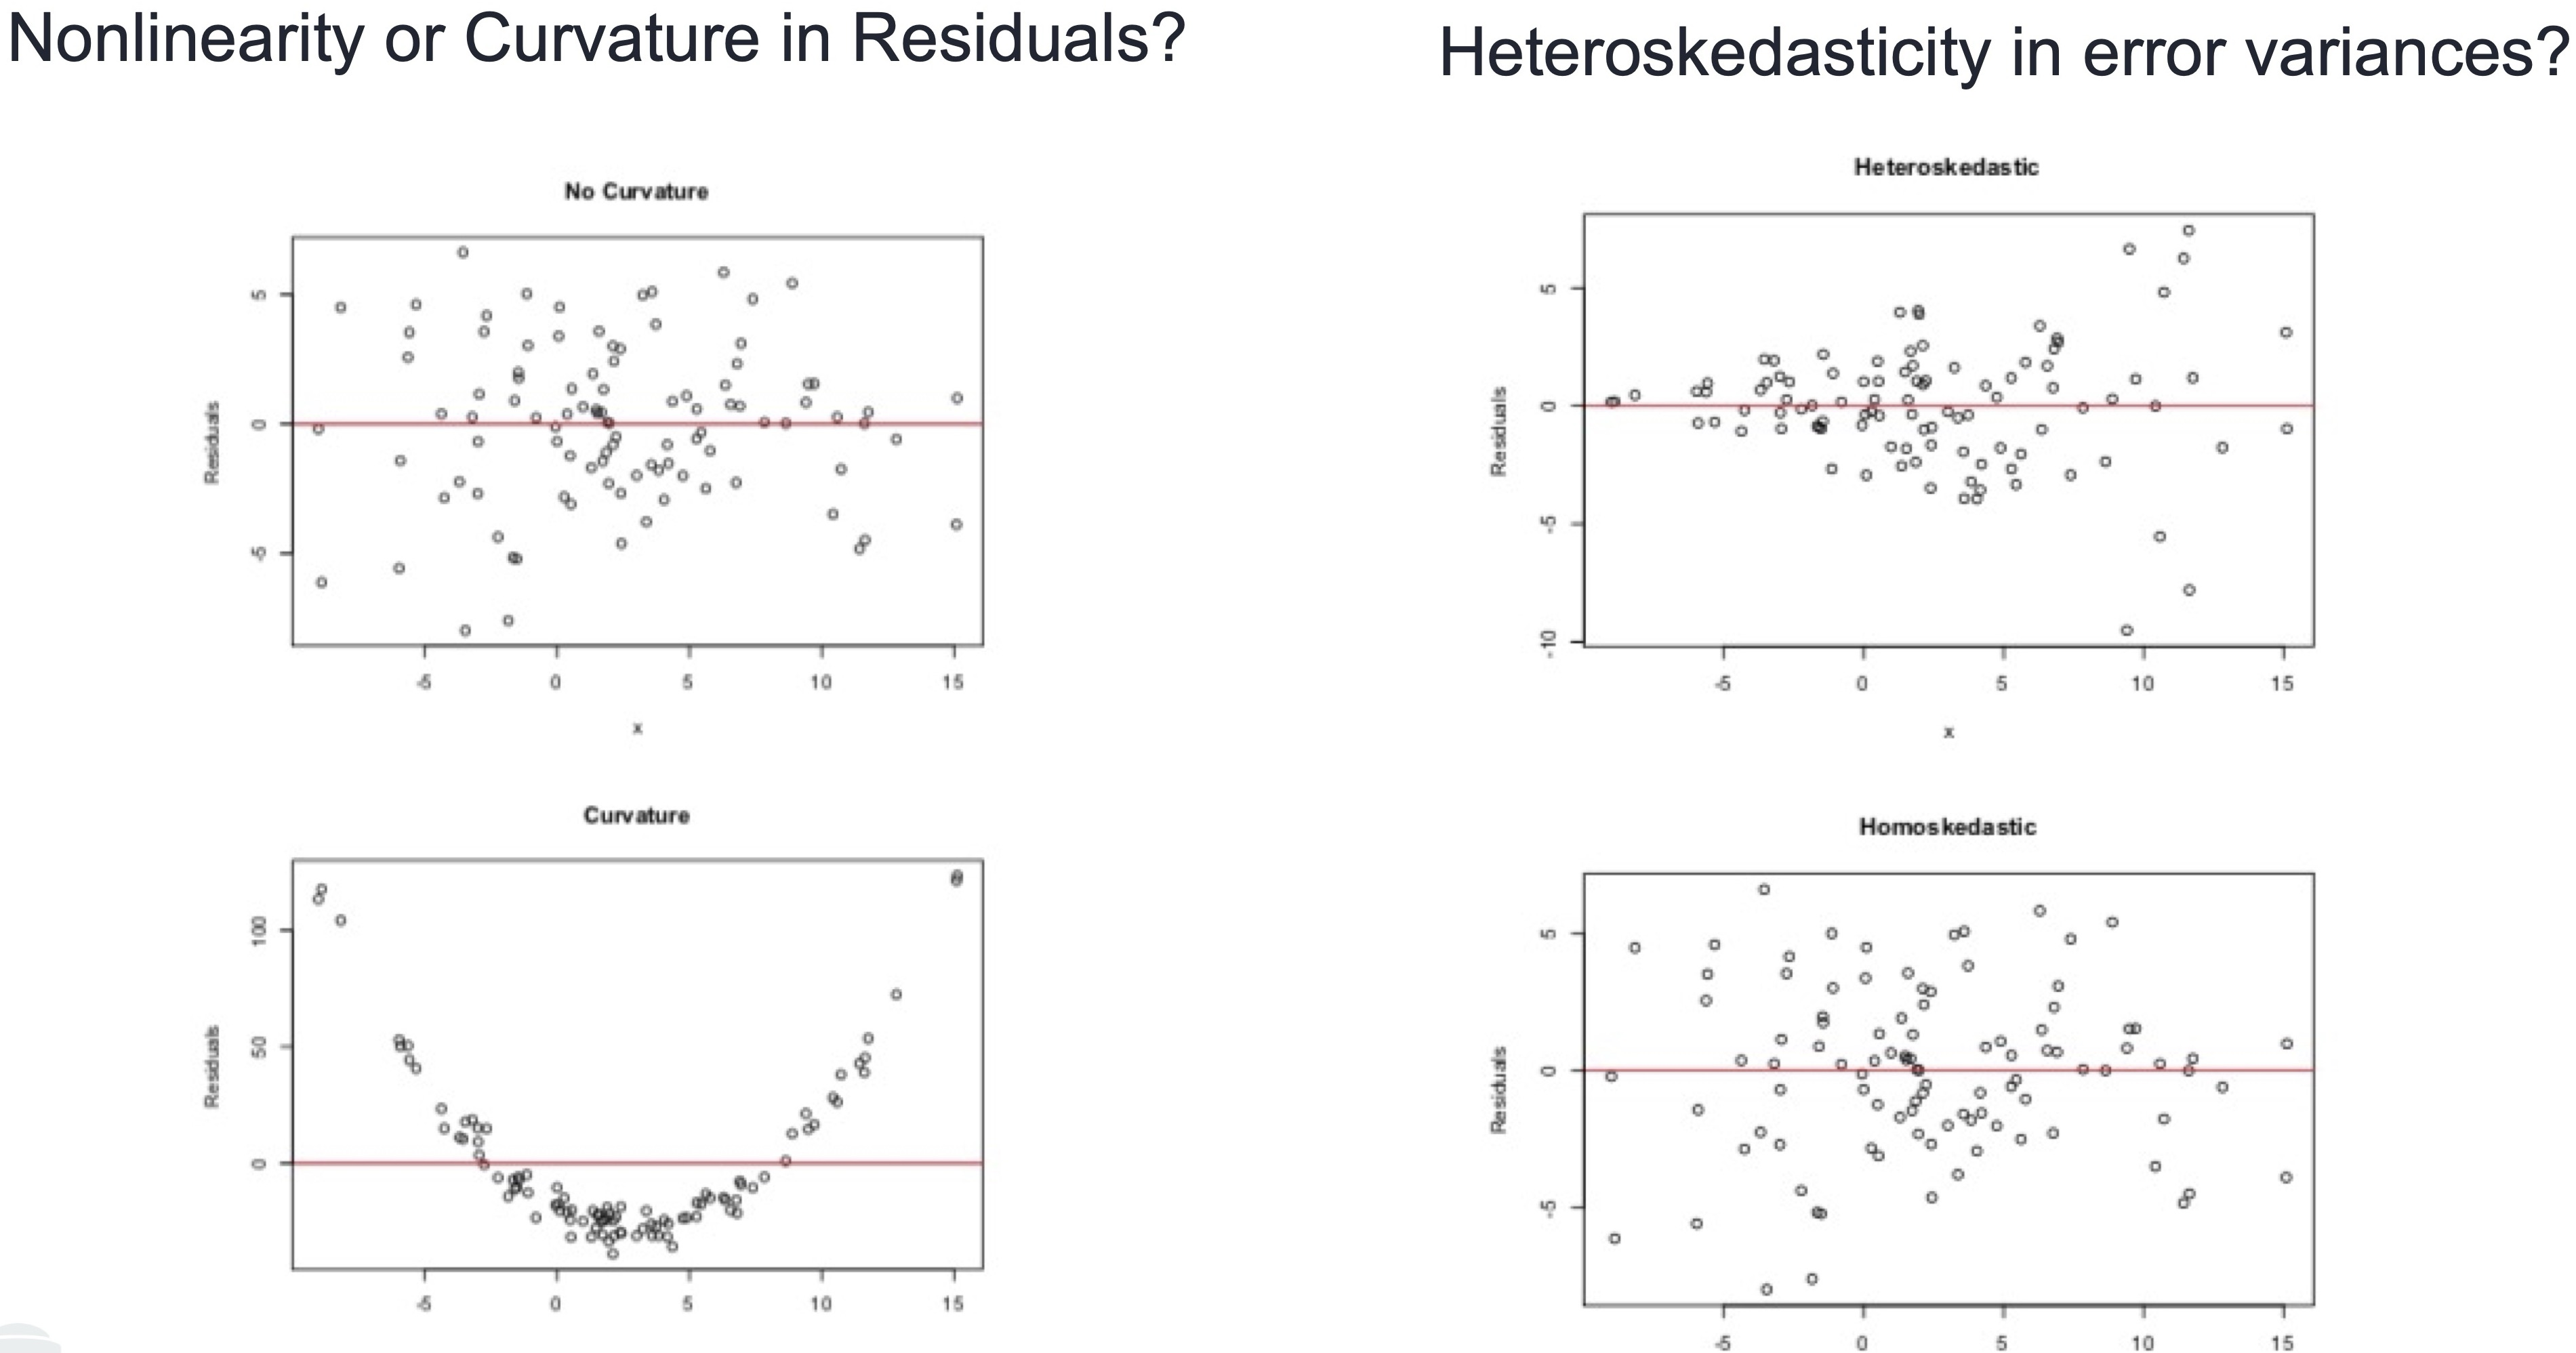
\includegraphics[width=0.25\textwidth]{residuals1.jpg}
Top-right: hetero. Bottom-right:homo.
\Green{Normality} the residuals are approximately normal.
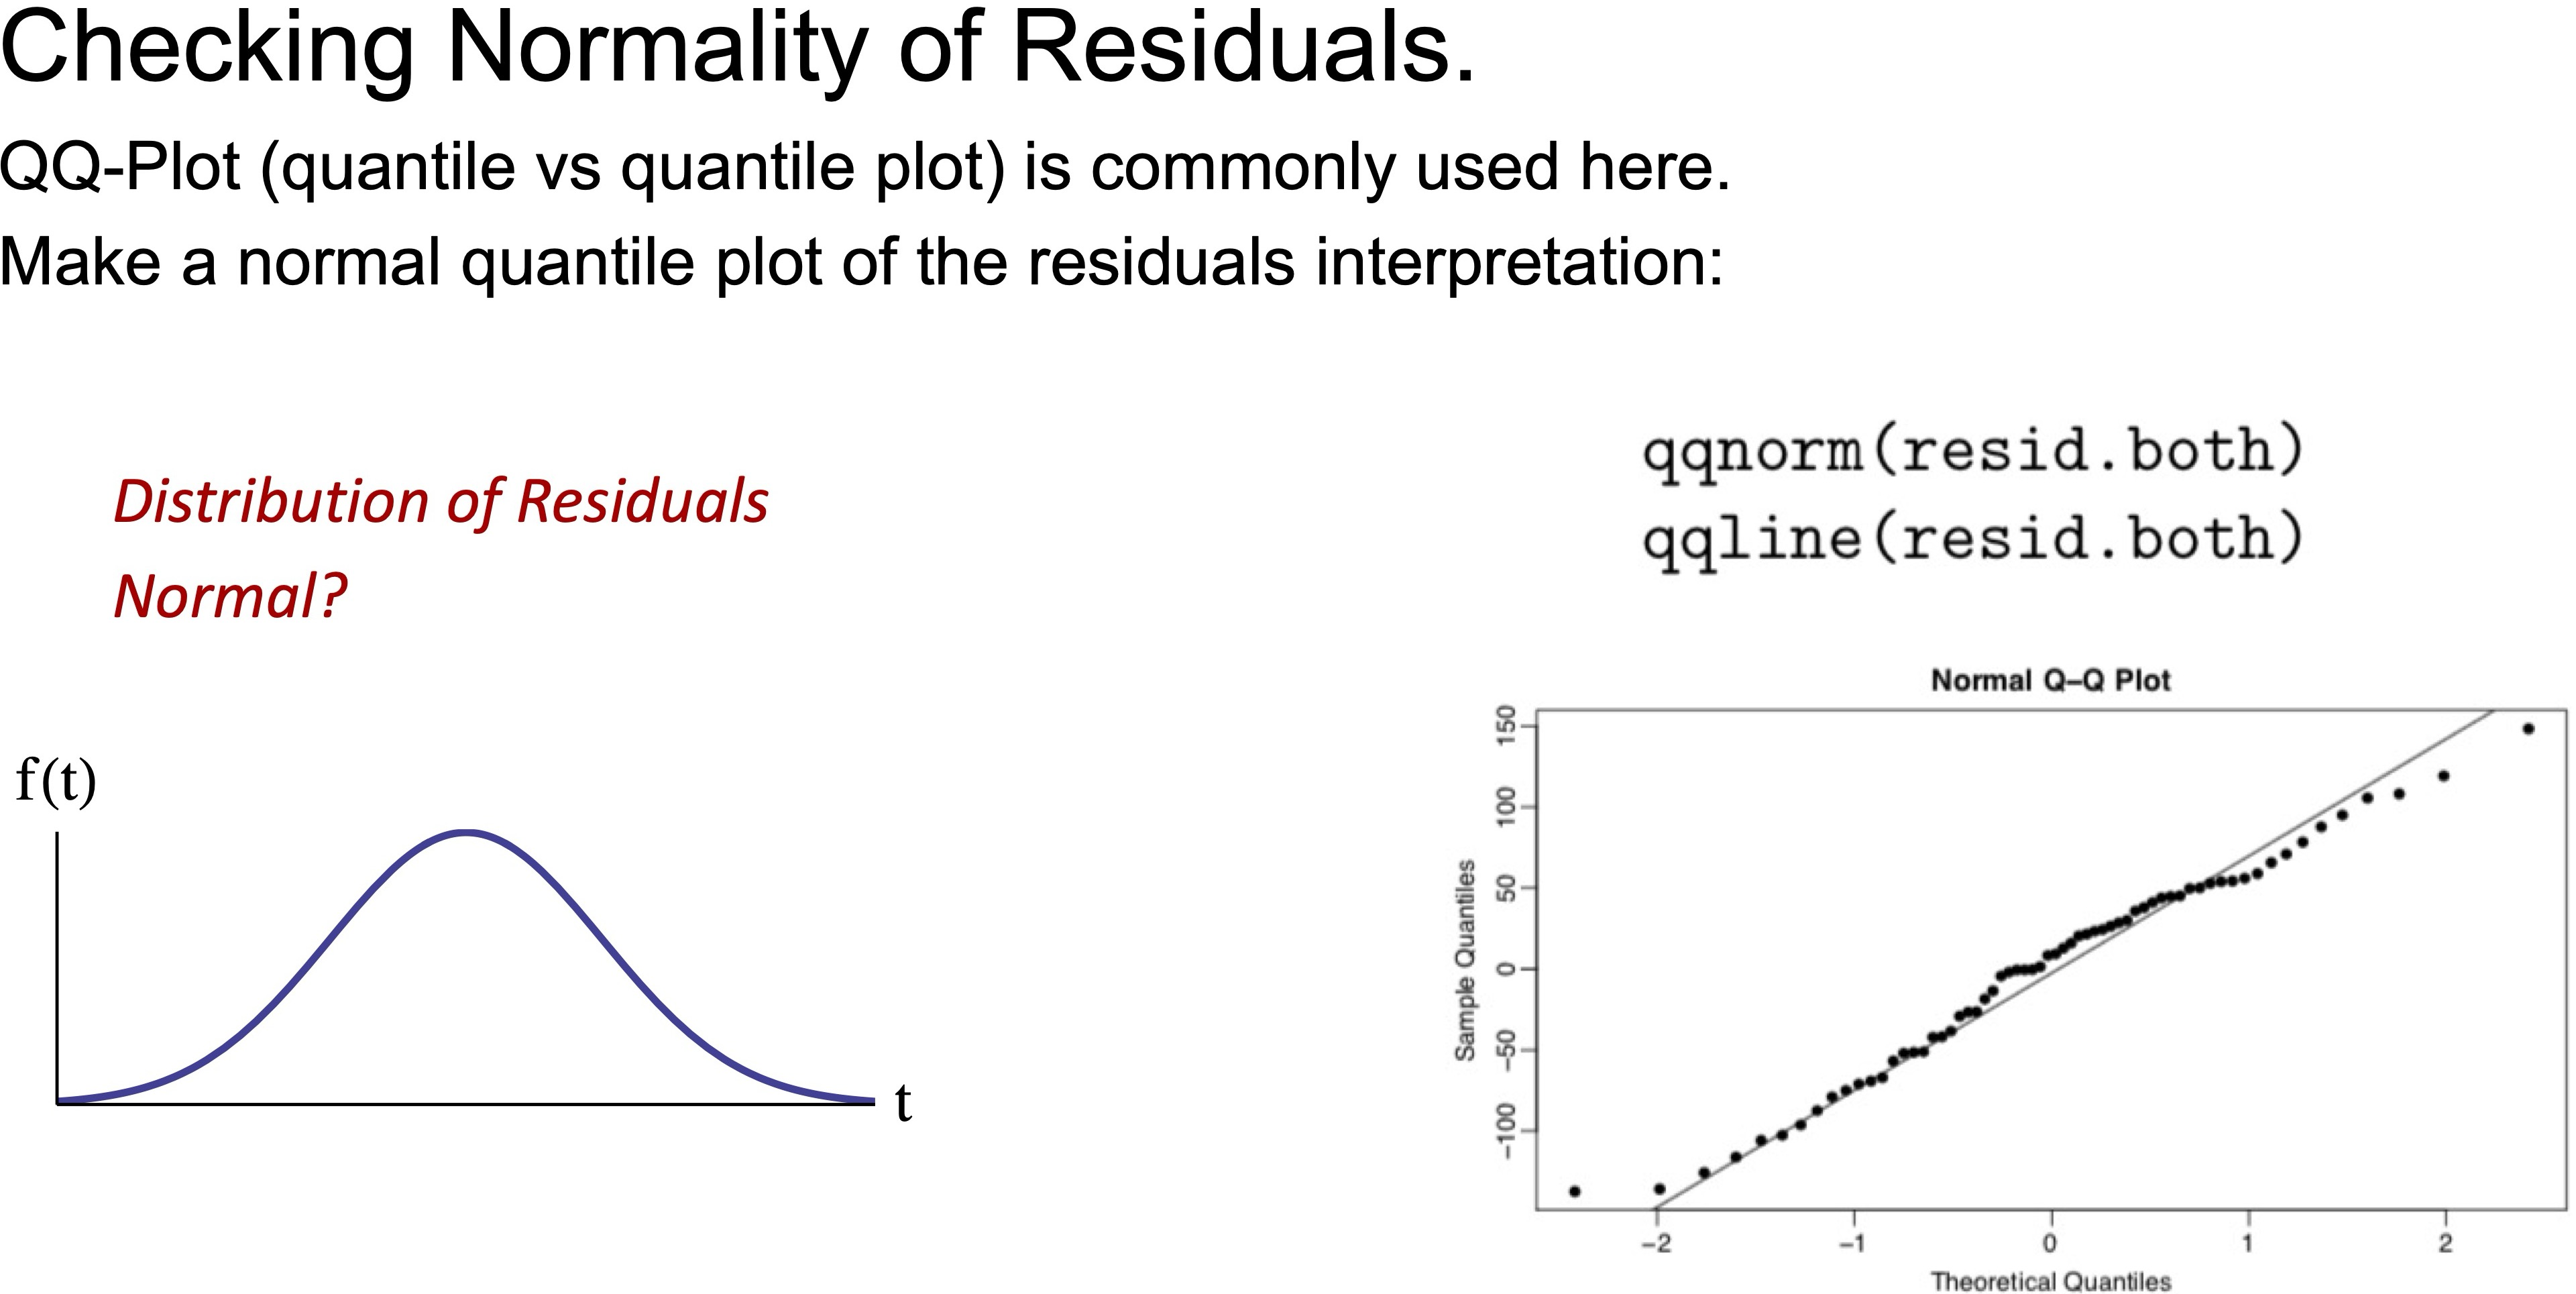
\includegraphics[width=0.25\textwidth]{residuals2.jpg}


\section{Side bar}

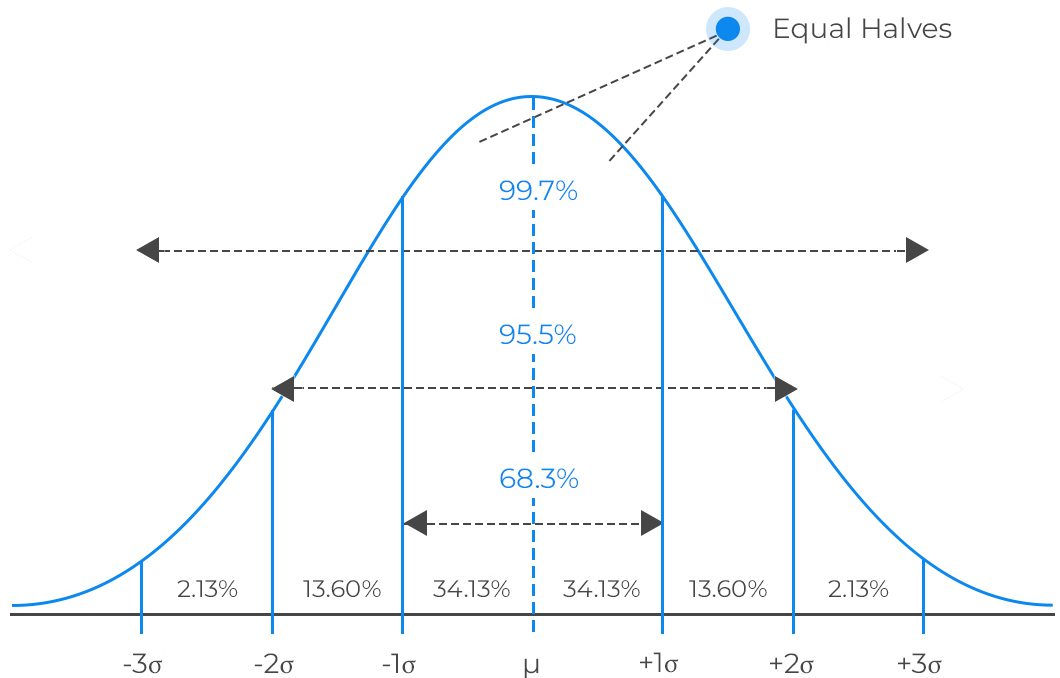
\includegraphics[width=0.25\textwidth]{normal_distribution_property.jpg}

\begin{itemize}
    \item about 68\% of the total values lie within 1 standard deviation of the mean. 
    \item about 95\% lie within 2 standard deviations of the mean
    \item about 99.7\% lie within 3 standard deviations of the mean.
\end{itemize}

\end{multicols}
\end{document}